\documentclass[a4paper,12pt]{article}
\usepackage[a4paper,top=1.3cm,bottom=2cm,left=1.5cm,right=1.5cm,marginparwidth=0.75cm]{geometry}
\usepackage{cmap}
\usepackage{mathtext}
\usepackage[T2A]{fontenc}
\usepackage[utf8]{inputenc}
\usepackage[english,russian]{babel}
\usepackage{siunitx}
\usepackage{enumitem}
\usepackage{placeins}

\usepackage{graphicx}

\usepackage{wrapfig}
\usepackage{tabularx}
\usepackage{multirow}

\usepackage{hyperref}
\usepackage[rgb]{xcolor}
\hypersetup{
colorlinks=true,urlcolor=blue
}
\usepackage{amsmath,amsfonts,amssymb,amsthm,mathtools}
\usepackage{icomma}
\mathtoolsset{showonlyrefs=false}
\usepackage{euscript}
\usepackage{mathrsfs}
\DeclareMathOperator{\sgn}{\mathop{sgn}}
\newcommand*{\hm}[1]{#1\nobreak\discretionary{}
{\hbox{$\mathsurround=0pt #1$}}{}}

%%% Заголовок
\author{Макаров Лев Евгеньевич}
\title{Лабораторная работа №3.5.1

Изучение плазмы газового разряда в неоне
}
\date{\today}

\begin{document}

\begin{titlepage}
	\begin{center}
		{\large МОСКОВСКИЙ ФИЗИКО-ТЕХНИЧЕСКИЙ ИНСТИТУТ (НАЦИОНАЛЬНЫЙ ИССЛЕДОВАТЕЛЬСКИЙ УНИВЕРСИТЕТ)}
	\end{center}
	\begin{center}
		{\large Физтех-школа фотоники, электроники и молекулярной физики}
	\end{center}
	
	
	\vspace{4.5cm}
	{\huge
		\begin{center}
			{\bf Отчёт о выполнении лабораторной работы 3.5.1}\\
			Изучение плазмы газового разряда в неоне
		\end{center}
	}
	\vspace{2cm}
	\begin{flushright}
		{\LARGE Автор:\\ Макаров Лев Евгеньевич \\
			\vspace{0.2cm}
			Б04-306}
	\end{flushright}
	\vspace{8cm}
	\begin{center}
		Долгопрудный 2024
	\end{center}
\end{titlepage}

\section{Введение}

\textbf{Цель работы:} 
\begin{enumerate}
	\item Исследование характеристик газового разряда
\end{enumerate}

\textbf{В работе используются:} 
\begin{itemize}
    \item стеклянная газоразрядная трубка, наполненная неоном
    \item высоковольтный источник питания
    \item источник питания постоянного тока
    \item делитель напряжения
    \item резистор
    \item потенциометр
    \item амперметры
    \item вольтметры
    \item переключатели
\end{itemize}
\medskip

\section{Теоретические сведения}

\subsection*{Плазма}
	
Из-за теплового движения в плазме электроны могут смещаться относительно ионов и образовывать неоднородности. В этих неоднородностях возникает электрическое поле, которое стремится восстановить баланс, из-за чего происходят колебания с частотой

\begin{equation*}
    w_p = \sqrt{\frac{4\pi n_e e^2}{m_e}}
\end{equation*}

За характерное время колебаний электроны за счет теплового движения смещаются на

\begin{equation*}
    r_D \sim \frac{v_e}{w_p} = \sqrt{\frac{kT_e}{4\pi n_e e^2}}    
\end{equation*}

$r_D$ - дебаевский радиус, $k$ - константа Больцмана.\\
Если поместить в плазму пробную (допустим, положительную) частицу, то электроны будут скапливаться около этой частицы, экранируя её поле. Потенциал точечного заряда будет иметь в плазме следующий вид:

\begin{equation*}
    \varphi(r) = \frac{q}{r}e^{-\frac{r}{r_D}}
\end{equation*}

где $r_D = \sqrt{\dfrac{kT_e}{4\pi n e^2}}$ -- \textit{радиус Дебая в случае равновесной плазмы}. Если температуры электронов и ионов сильно отличаются, то следует определять отдельно величину радиуса экранирования для электронов и для ионов. Итоговый радиус будет

\begin{equation*}
    r_D = (r_{De}^{-2} + r_{Di}^{-2})^{-1/2}
\end{equation*}

То есть если $T_i \ll T_e$, то $r_D \approx r_{Di}$ 

\subsection*{Одиночный зонд}

При внесении в плазму уединённого проводника -- \textit{зонда} -- с потенциалом, изначально равным потенциалу точки плазмы, в которую его помещают, на него поступают токи электроннов и ионов:

\begin{equation}
    \begin{array}{c}
        I_{e0} = \dfrac{n \langle v_e \rangle}{4}eS,\\
        I_{i0} = \dfrac{n \langle v_i \rangle}{4}eS,
    \end{array}
\end{equation}

где $\langle v_e \rangle$ и $\langle v_i \rangle$ -- средние скорости электронов и ионов, $S$ -- площадь зонда, $n$ -- плотность электронов и ионов. Скорости электронов много больше скорости ионов, поэтому $I_{i0} \ll I_{e0}$. Зонд будет заряжаться до некоторого равновестного напряжения $-U_f$ -- \textit{плавающего потенциала}.\\
В равновесии ионный ток мало меняется, а электронный имеет вид

\begin{equation*}
    I_e = I_0 \exp\left( -\dfrac{eU_f}{kT_e} \right).
\end{equation*}


Будем подавать потенциал $U_\text{з}$ на зонд и снимать значение зондового тока $I_\text{з}$. Максимальное значение тока $I_{e\text{н}}$ -- электронный ток насыщения, а минимальное $I_{i\text{н}}$ -- ионный ток насыщения. Значение из эмпирической формулы Бомона:

\begin{equation}
    I_{i\text{н}} = 0.4 neS \sqrt{\dfrac{2kT_e}{m_i}}.
\end{equation}
	
Электронный ток насыщения можно определить по тепловому движению:

\begin{equation*}
    I_{e\text{н}} = \frac{n_eS}{4}\sqrt{\frac{8kT}{\pi m_e}}  
\end{equation*}

\subsection*{Двойной зонд}

Двойной зонд -- система из двух одинаковых зондов, расположенных на небольшом расстоянии друг от друга, между которыми создаётся разность потенциалов, меньшая $U_f$. Рассчитаем ток между ними вблизи $I=0$. При небольших разностях потенциалов ионные токи на оба зонда близки к току насыщения и компенсируют друг друга, а значит величина результирующего тока полностью связана с разностью электронных токов. Пусть потенциалы на зондах

\begin{equation*}
    U_1 = -U_f + \Delta U_1,
\end{equation*}


\begin{equation*}
    U_2 = -U_f + \Delta U_2.
\end{equation*}

Между зондами $U = U_2 - U_1 = \Delta U_2 - \Delta U_1$.
Через первый электрод

\begin{equation}
    I_1 = I_{i\text{н}} + I_{e1} = I_{i\text{н}} - \dfrac{1}{4}neS\langle v_e\rangle \exp\left(-\dfrac{eU_f}{kT_e}\right)\exp\left(\dfrac{e\Delta U_1}{kT_e}\right)=I_{i\text{н}}\left(1 - \exp\left( \dfrac{e\Delta U_1}{kT_e} \right)\right).
\end{equation}

Аналогично через второй получим

\begin{equation}
    I_2 = I_{i\text{н}}\left(1 - \exp\left( \dfrac{e\Delta U_2}{kT_e} \right)\right)
\end{equation}
	
Из $(7)$ и $(8)$ с учётом последовательного соединение зондов ($I_1 = -I_2 = I)$:

\begin{equation*}
    \Delta U_1= \dfrac{kT_e}{e}\text{ln}\left(1 - \dfrac{I}{I_{i\text{н}}}\right)
\end{equation*}

\begin{equation*}
    \Delta U_2= \dfrac{kT_e}{e}\text{ln}\left(1 + \dfrac{I}{I_{i\text{н}}}\right)
\end{equation*}

Тогда итоговые формулы для разности потенциалов и тока
	
\begin{equation}
    U = \dfrac{kT_e}{e}\text{ln}\dfrac{1 - I/I_{i\text{н}}}{1 + I/I_{i\text{н}}}, \ \
    I = I_{i\text{н}} \text{th}\dfrac{eU}{2kT_e}.
\end{equation}

\begin{wrapfigure}[5]{l}{0.4\textwidth}
    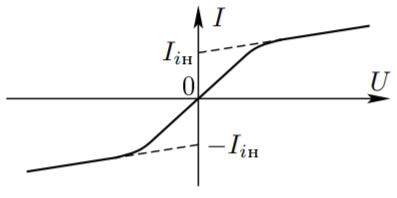
\includegraphics[scale=0.8]{vah-theory.png}
\end{wrapfigure}

Зависимость выглядит примерно так.
Из формулы можно найти формулу для $T_e$: для $U=0$ мы найдём $I_{i\text{н}}$, продифференцируем в точке $U=0$ и с учётом $\text{th}~\alpha \approx \alpha$ при малых $\alpha$ и $A\rightarrow 0$ получим:

\begin{equation}
    kT_e = \dfrac{1}{2}\dfrac{eI_{i\text{н}}}{\dfrac{dI}{dU}|_{U=0}}.
\end{equation}

\section{Экспериментальная установка}

\begin{center}
    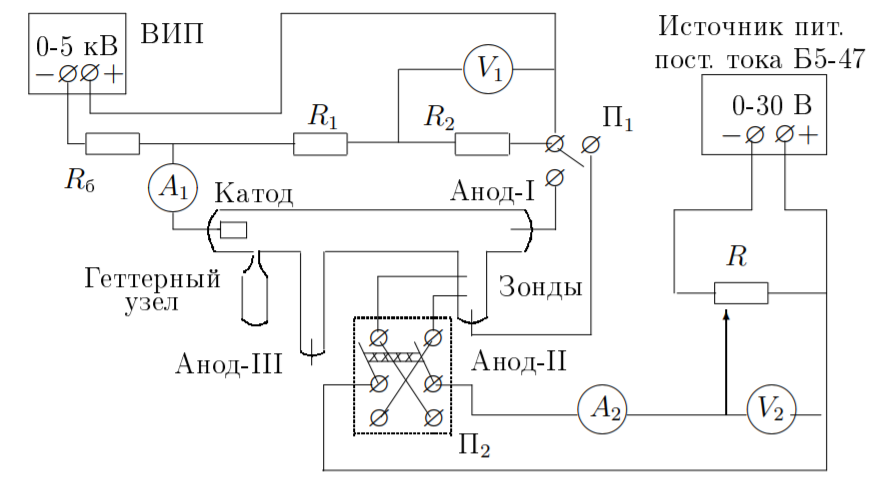
\includegraphics[scale=0.9]{ust-1.png}
\end{center}

Стеклянная газоразрядная трубка имеет холодный (ненакаливаемый) полый катод, три анода и \textit{геттерный} узел -- стеклянный баллон, на внутреннюю повехность которого напылена газопоглощающая плёнка (\textit{геттер}). Трубка наполнена изотопом неона $^22$Ne при давлении 2 мм рт. ст. Катод и один из анодом (I и II) с помощью переключателя $\Pi_1$ подключается через балластный резистор $R_\text{б}$ ($\approx 450$ кОм) к регулируемому ВИП с выкодным напряжением до 5 кВ.\\

При подключении к ВИП анода-I между ним и катодом возникает газовый разряд. Ток разряда измеряется миллиамперметром $A_1$, а падение напряжения на разрядной трубке -- цифровым вольтметром $V_1$, подключённым к трубке черезе высокоомный (25 МОм) делитель напряжения с коэффициентом $(R_1+R_2)/R_2 = 10$.\\

При подключении к ВИП анода-II разряд возникает в пространстве между катодом и анодом-II, где находятся двойной зонд, используемый для диагностики плазмы положительного столба. Зонды изготовлены из молибденовой проволоки диаметром $d = 0.2$ мм и имеют длину $l = 5.2$ мм. Они подключены к источнику питания GPS через потенциометр $R$. Переключатель $\Pi_2$ позволяет изменять полярность напряжения на зондах. Величина напряжения на зондах изменяеься с помощью дискретного переключателя <<$V$>> выходного напряжения источника питания и потенциометра $R$, а измеряется цифровым вольтметром $V_2$. Для измерения зондового тока используется мультиметр $A_2$.

\section{Результаты измерений и обработка данных}

\section*{ВАХ разряда}

\begin{enumerate}
    \item Подготовим все приборы к работе.
\end{enumerate}
Включим в сеть ВИП и мультиметр $V_1$. Будем плавно увеличивать выходное напряжение ВИП с нулевого значения до того момента, как в трубке зажжётся разряд. Показания вольтметра $V_1$ непосредственно перед зажиганием -- т.н. напряжение зажигания разряда -- равны $U_{\text{заж}}=\left(231\pm3\right)~\text{В}$.

\begin{enumerate}[resume]
    \item С помощью вольтметра $V_1$ и амперметра $A_1$ снимем вольт-амперную характеристику разряда $U_{\text{р}}\left(I_{\text{р}}\right)$ в диапазоне от $0,5~\text{мА}$ до $\approx5~\text{мА}$ по току.
\end{enumerate}
Измерения проведём как при нарастании ($\nearrow$), так и при убывании ($\searrow$) тока. Занесём полученные данные в таблицу \Ref{VAH}. Заметим заранее, что гистерезиса ВАХ в работе не наблюдается, поэтому при построении графика имеет смысл использовать значения, полученные при усреднении ($\langle\ldots\rangle$) снятых значений. Тоже занесём эти точки в таблицу.

Оценим также погрешности. Погрешность амперметра $A_1$ равна половине цены его деления, $\Delta I=0,02~\text{мА}$. Погрешность вольтметра равна $0,003U+4~\text{ед. мл. разряда}$.


\begin{table}[h]
	\centering
	\caption{Зависимость тока разряда $I_{\text{р}}$ от его напряжения $U_{\text{р}}$ при нарастании и убывании} \label{VAH}
	\begin{tabular}{|c|c|c|c|c|c|c|c|c|}
		\hline
        $U_{\text{р}}^\text{возр}$, В & 26,02 & 22,96 & 22,86 & 22,11 & 22,45 & 23,14 & 24,49 & 35,37 \\ \hline
		$I_{\text{р}}$, мА & 0,5 & 0,8 & 1,1 & 1,4 & 1,7 & 2,0 & 2,3 & 2,6 \\ \hline \hline
		$U_{\text{р}}^\text{убыв}$, В & 24,9 & 23,12 & 22,0 & 22,11 & 22,74 & 22,9 & 26,29 & ~ \\ \hline
        $I_{\text{р}}$, мА & 2,3 & 2,0 & 1,7 & 1,4 & 1,1 & 0,8 & 0,5 & ~ \\ \hline
	\end{tabular}
\end{table}

Построим вольт-амперную характеристику разряда в координатах $I_{\text{р}}\left(U_{\text{р}}\right)$. Она представлена на рисунке \Ref{Zond_VAH}. По наклону кривой на левом конце графика определим минимальное дифференциальное сопротивление разряда $R_{\text{диф}}\equiv\frac{\text{d}U}{\text{d}I}= 36000 ~\Omega$. Сравнив график с рисунком \Ref{Characteristic} (в Приложении к отчёту), сделаем вывод, что полученный в работе график \textit{соответствует участку Г--Д}.

\begin{figure}[h]
	\centering
	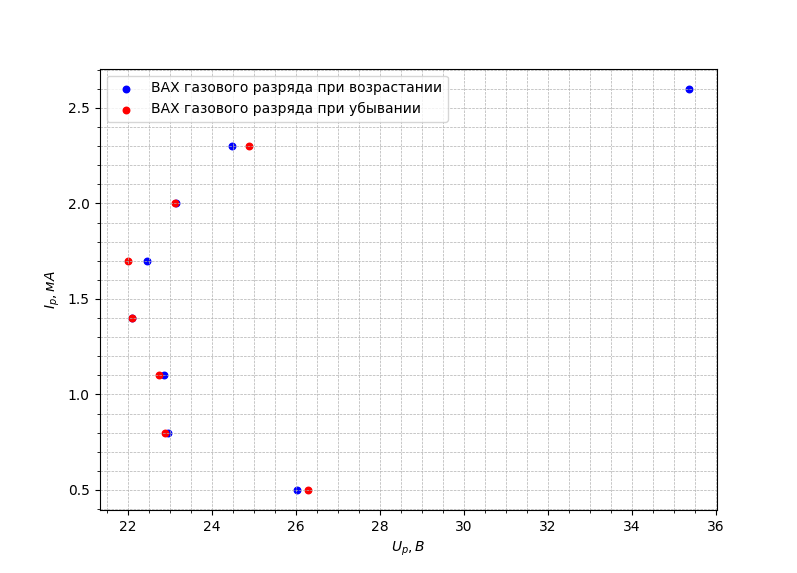
\includegraphics[scale=0.9]{8.png}
	\caption{Вольт-амперная характеристика разряда $I_{\text{р}}\left(U_{\text{р}}\right)$. Сглаживающая кривая проведена с помощью кубического сплайна} \label{Zond_VAH}
\end{figure}

\FloatBarrier
\subsection*{II. Зондовые характеристики}

Подготовим приборы к работе. Плавно увеличим напряжение ВИП до возникновения разряда. Установим максимально допустимое значение разрядного тока $I_{\text{р}}^{max}=5,0~\text{мА}$. Подготовим к работе источник питания, после чего с помощью потенциометра $R$ установим на зонда максимально допустимое напряжение $U_{\text{з}}^{max}=25,0~\text{В}$.

Измерим вольт-амперную характеристику двойного зонда $I_{\text{з}}\left(U_{\text{з}}\right)$ в диапазоне от $-U^{max}_{\text{з}}$ до $U^{max}_{\text{з}}$ при фиксированном токе разряда $I_{\text{р}}$. Проведём данные измерения при трёх различных значениях тока разряда ($2,0~\text{мА}$, $1,5~\text{мА}$ и $0,84~\text{мА}$ в таблице соответственно). Занесём полученные данные в таблицу \Ref{Holl}. Отцентрируем кривую: проведём ось абсцисс на уровне $I=\frac{1}{2}\sum\Delta I$ и восстановим ось ординат из точки пересечения кривой с осью абсцисс. Пересчитанные для этого точки с индексом $c$ также занесём в таблицу.

\begin{table}[h]
	\centering
	\caption{Зависимость напряжения на зонде $U_{\text{з}}$ от тока $I_{\text{з}}$ через него значениях $I_{\text{р}}=2,0~\text{мА},\ 1,5~\text{мА}\ \text{и}\ 0,84~\text{мА}$ соответственно} \label{Holl}
	\begin{tabular}{|c|c|c|c|c|c|c|c|c|c|}
		\hline
		$U_{\text{з}},\text{В}$ && $I_{\text{з}},\text{мкА}$ & $I_{\text{з}c},\text{мкА}$ && $I_{\text{з}},\text{мкА}$ & $I_{\text{з}c},\text{мкА}$ && $I_{\text{з}},\text{мкА}$ & $I_{\text{з}c},\text{мкА}$ \\ \hline
		25,0 && 39,8 & 37,1 && 77,8 & 73,3 && 124,0 & 118,0 \\ \hline
		22,0 && 38,4 & 35,7 && 75,6 & 71,1 && 127,1 & 121,1 \\ \hline
		19,0 && 37,1 & 34,4 && 73,4 & 68,9 && 125,4 & 119,4 \\ \hline
		16,0 && 35,8 & 33,1 && 70,1 & 65,6 && 121,4 & 115,4 \\ \hline
		13,0 && 34,1 & 31,4 && 67,2 & 62,7 && 113,1 & 107,1 \\ \hline
		10,0 && 31,1 & 28,4 && 60,5 & 56,0 && 99,4 & 93,4 \\ \hline
		8,0 && 27,9 & 25,2 && 53,6 & 49,1 && 86,4 & 80,4 \\ \hline
		6,0 && 23,4 & 20,7 && 44,5 & 40,0 && 69,9 & 63,9 \\ \hline
		4,0 && 17,5 & 14,8 && 32,4 & 27,9 && 49,2 & 43,2 \\ \hline
		2,0 && 10,1 & 7,4 && 18,3 & 13,8 && 24,9 & 18,9 \\ \hline
		0,0 && 2,7 & 0,0 && 4,5 & 0,0 && 6,0 & 0,0 \\ \hline
		-2,0 && -5,6 & -8,3 && -9,9 & -14,4 && -12,5 & -18,5 \\ \hline
		-4,0 && -12,9 & -15,6 && -24,0 & -28,5 && -36,8 & -42,8 \\ \hline
		-6,0 && -18,7 & -21,4 && -35,7 & -40,2 && -57,6 & -63,6 \\ \hline
		-8,0 && -23,0 & -25,7 && -44,9 & -49,4 && -74,8 & -80,8 \\ \hline
		-10,0 && -25,9 & -28,6 && -51,6 & -56,1 && -87,8 & -93,8 \\ \hline
		-13,0 && -28,6 & -31,3 && -57,9 & -62,4 && -101,4 & -107,4 \\ \hline
		-16,0 && -30,1 & -32,8 && -61,4 & -66,1 && -109,4 & -115,4 \\ \hline
		-19,0 && -31,2 & -33,9 && -63,7 & -68,2 && -113,1 & -119,1 \\ \hline
		-22,0 && -32,4 & -35,1 && -65,7 & -70,2 && -114,8 & -120,8 \\ \hline
		-25,0 && -33,5 & -36,2 && -67,7 & -72,2 && -112,2 & -118,2 \\ \hline
	\end{tabular}
\end{table}

\FloatBarrier
\begin{figure}[h]
	\centering
	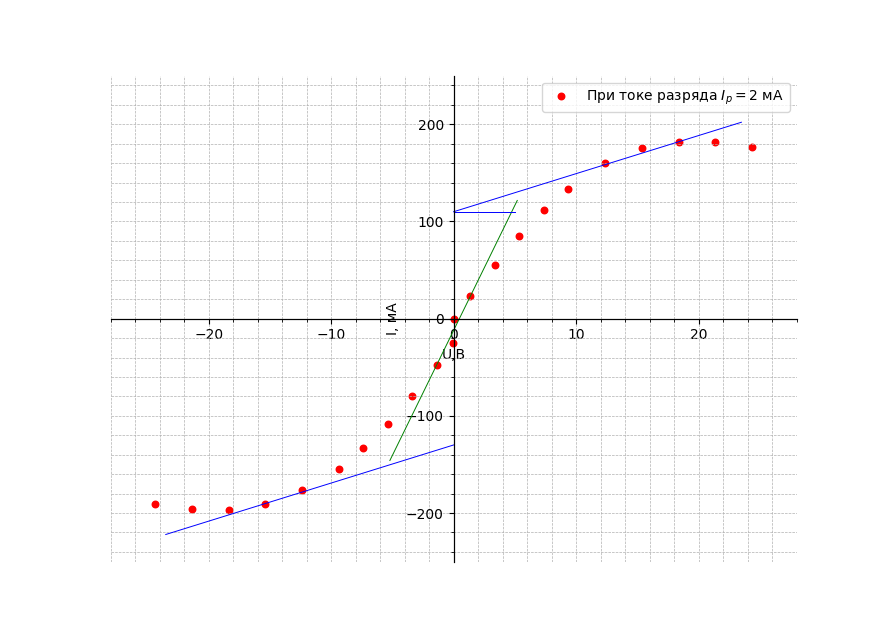
\includegraphics[scale=0.9]{vah-2ma.png}
	\caption{Зондовая характеристика через разряд $I_{\text{р}} = 2,00$ мА}
    \label{vah-2}
\end{figure}
\FloatBarrier
\begin{figure}[h]
	\centering
	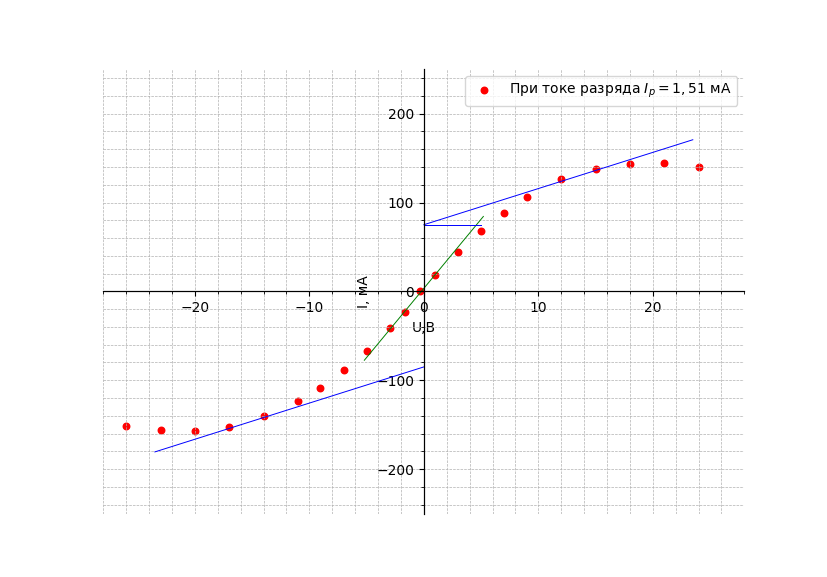
\includegraphics[scale=0.9]{vah-151ma.png}
	\caption{Зондовая характеристика через разряд $I_{\text{р}} = 1,51$ мА}
    \label{vah-151}
\end{figure}
\FloatBarrier
\begin{figure}[h]
	\centering
	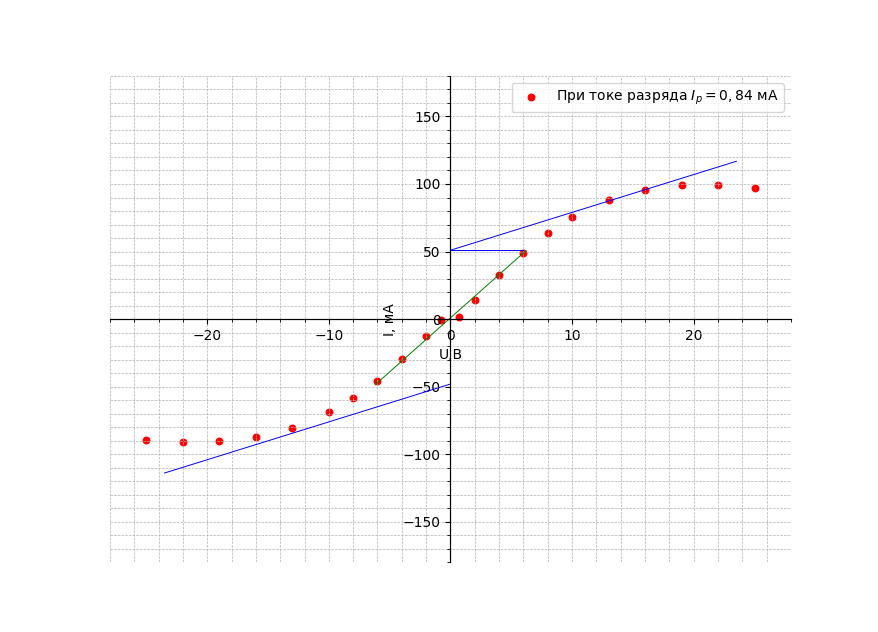
\includegraphics[scale=0.9]{vah-084ma.png}
	\caption{Зондовая характеристика через разряд $I_{\text{р}} = 0,84$ мА}
    \label{vah-084}
\end{figure}
\FloatBarrier
\begin{figure}[h]
	\centering
	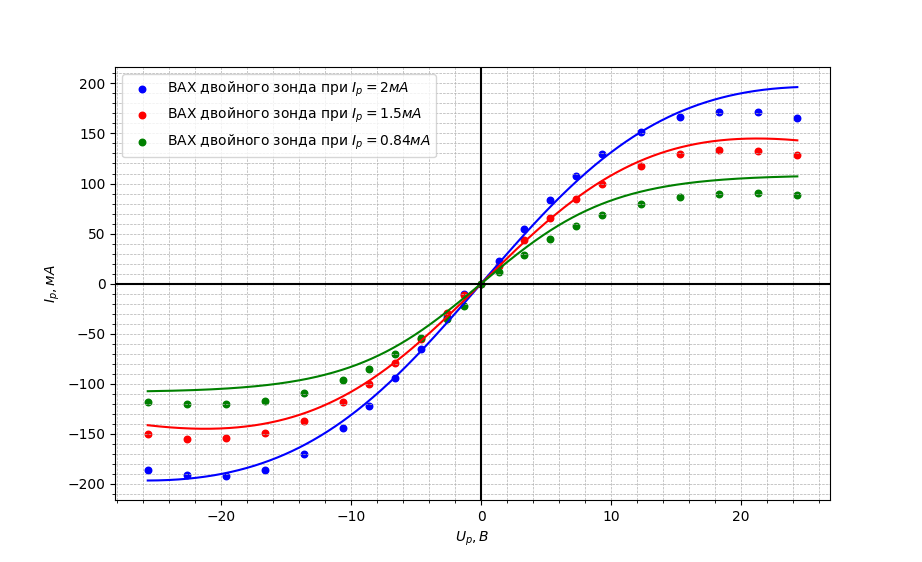
\includegraphics[scale=0.9]{vah-all.png}
	\caption{Зондовые характеристики через разряд}
    \label{vah-all}
\end{figure}
\FloatBarrier

По графикам определим температуру электронов. 

\begin{equation*}
    kT_e=\frac{e\Delta U}{2}
\end{equation*}

$kT_e = \dfrac{1}{2}\dfrac{eI_{i\text{н}}}{\dfrac{dI}{dU}|_{U=0}}.$\\
$kT_e = \frac{\Delta U}{2}$, где $\Delta U$ - расстояние между точками 1 и 2.\\
$I_{i\text{н}} = 0.4 neS \sqrt{\dfrac{2kT_e}{m_i}}.$, где S=$\pi$dl - площадь поверхности зонда. Зная, что d=0,2 мм, l=5,2 мм,\\ получим S=$3,27*10^{-6} м^2$, а $m_i$= $22*1,66*10^{-27} кг$- масса иона неона.\\
$\omega_p = \sqrt{\dfrac{4\pi ne^2}{m}}=5,6*10^4*\sqrt{n_e} \frac{рад}{с}$ - плазменная частота колебаний электронов.\\

$r_D = \sqrt{\dfrac{kT_e}{4\pi n e^2}}$ -радиус Дебая. Среднее число ионов в сфере такого радиуса $N_D = n\dfrac{4}{3}\pi r_D^2.$\\

\begin{table}[!ht]
    \centering
    \begin{tabular}{|l|l|l|l|l|l|l|l|l|l|}
    \hline
        $I_p, мА$ & $I_{in}, мА$ & dI/dU, мА/В & kT, Эв & T,К*$10^3 $& $n_e, 10^{16}, v^{-3}$ & $\omega 10^{12} рад/с$& r_d 10^{-4} м & $N_d, 10^5$ & $\alpha$ \\ \hline
        2 & 110 & 25,73 & 3 & 35,4 & 3,76 & 10,85880288 & 6 & 3,25 & ~ \\ \hline
        1,5 & 75 & 3,4 & 2,5 & 41,3 & 3,45 & 10,4 & 6,60 & 3,97 & ~ \\ \hline
    \end{tabular}
    \caption{Данные расчетов}
\end{table}

Графики зависимости Te(Ip),ne(Ip) занесены на Рисунок 6.\\

\begin{figure}[!ht]
\begin{center}
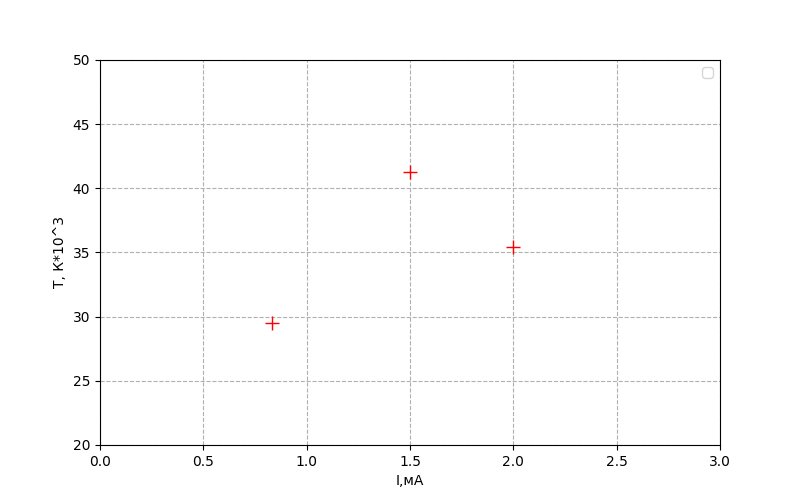
\includegraphics[scale=0.6]{rty1.png}
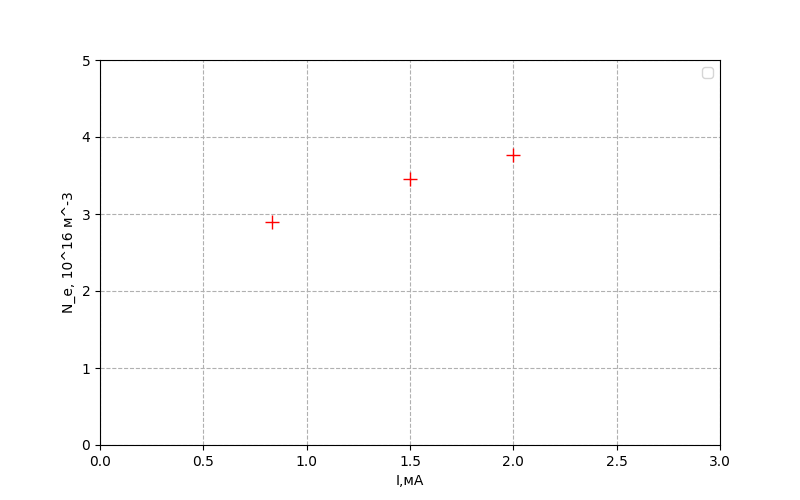
\includegraphics[scale=0.6]{кен2.png}
\caption{Графики зависимости Te(Ip),ne(Ip)}
\end{center}
\end{figure}	

\section{\Large{Вывод}}
В данной лабораторной работе мы исследовали состояние плазмы в тлеющем газовом разряде c помощью двойного зонда. Полученные результаты сходятся с указанными в лабораторной работе по порядку. Плазму в тлеющем разряде можно с хорошей точностью назвать идеальной, так как $N_D > 30 \gg 1$.


\end{document}
